\chapter{Multi-Agent-SCADA Systeme}
\label{cha:scadasysteme}

Obwohl es verschiedenste Literatur über Multi-Agent-Systeme gibt, wird der Begriff \textit{Agent} nicht einheitlich definiert.
In dieser Arbeit wird unter diesen Terminus ein Softwareprozess mit folgenden Eigenschaften verstanden \cite{wooldridge_jennings_1995}:

\begin{itemize}
    \item Autonomie: Agenten agieren ohne direktes Eingreifen von Menschen oder anderen und haben eine gewisse Kontrolle über ihre Handlungen und ihren internen Zustand.
    \item Soziale Fähigkeit: Agenten interagieren mit anderen Agenten (und möglicherweise Menschen) über eine Art von Agenten-Kommunikationssprache.
    \item Reaktivität: Agenten nehmen ihre Umgebung wahr (das kann die physische Welt, ein Benutzer über eine grafische Benutzeroberfläche, eine Sammlung anderer Agenten, das Internet oder alles zusammen sein) und reagieren zeitnah auf Veränderungen in dieser Umgebung.
    \item Proaktivität: Agenten handeln nicht nur in Reaktion auf ihre Umwelt, sondern sind in der Lage, zielgerichtetes Verhalten an den Tag zu legen, indem sie die Initiative ergreifen.
\end{itemize}

Ein Multi-Agent-System kann daher als Sammlung von miteinander interagierenden Agents interpretiert werden \cite{MultiagentSystems}.

\section{Verwendung zur Digitalisierung von Fabriken}



\section{Simatic Windows Control Center Open Architecturee}

Das Basissystem WinCC Open Architecture stellt eine Umgebung zum Erstellen solcher Systeme zur verfügung und
eignet sich daher zum lösen komplexer Probleme. Es kann dazu verwendet werden um sich mit Teilnehmer in der Feldebene 
zu Verbinden, die Daten die diese Produzieren zu akquirieren und für Supervision verwenden. Es ist ein Vernetzen von bis zu 2048 Systemen möglich, dadurch kann man eine rekursive Systemtopologie erstellen, 
die ein Skalieren von Projekten ermöglicht. Außerdem kann man einzelne Agents über Rechnergrenzen hinweg verteilen.

\subsection{Projektaufbau und Hierarchie}

\subsection{Aufbau Datenbank}

Die 

\subsubsection{Datenpunkt Typen}

\begin{figure}[h]
	\centering 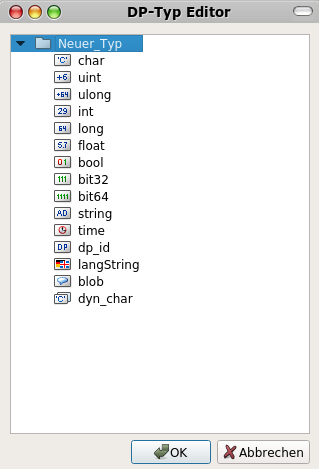
\includegraphics[width=0.40\textwidth]{dp_type}
	\caption{}
	\label{fig:dp_type}
\end{figure}

Die in Abbildung \ref{fig:dp_type}

\subsubsection{Datenpunkte}

\begin{figure}[h]
	\centering 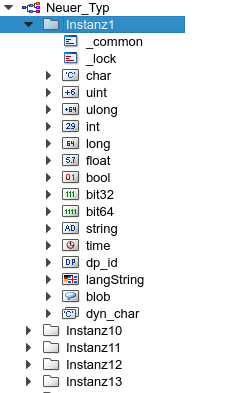
\includegraphics[width=0.35\textwidth]{dp_instances}
	\caption{}
	\label{fig:dp_instances}
\end{figure}

Die in Abbildung \ref{fig:dp_instances}

\subsubsection{Value Archive}

\subsection{Basis Agents und Konzept}

Je nach SCADA Produkt und Literatur werden die Teilnehmer eines solchen Systems unterschiedlich bezeichnet.
Während in dieser Arbeit der Begriff \textit{Agent} nach \cite{wooldridge_jennings_1995} Verwendung findet,
werden diese in WinCC OA als \textit{Manager} bezeichnet. Beide Begriffe folgen der vorher erläuterten Definition
für \textit{Agent}. Im kommenden Abschnitt werden die Basisprozesse eines WinCC OA Projekts beschrieben. 
Es wird dafür Bezug auf \cite{WinCCOA} genommen.

\subsubsection{Prozessmonitor}

Der Prozessmonitor startet und stoppt einzelne Prozesse eines WinCC OA Projektes und überwacht deren Status über zyklische
Anfragen. Im Fehlerfall versucht er den Prozess neu zu starten um somit ein stabiles gesamtsystem aufrecht zu erhalten.

\subsubsection{Event Manager}
Vermittelt anfragen etc.

\subsubsection{Data Manager}
Persistieren von Daten etc.

\subsubsection{Value Archive}
Historisches aufzeichnen von daten etc.

\subsubsection{Driver Manager}
Kommunizieren mit sps etc.

\subsubsection{Dist Manager}

\subsubsection{Redu Manager}

\subsubsection{API-Manager}

API

\subsection{C++-API}

WinCC OA stellt eine C++ Programmierschnittstelle zur Verfügung, mit der man eigene API Manager erstellen kann. 
Die Hauptfunktionen sind innerhalb zweier Singleton Klassen gekapselt.

\subsubsection{Manager Klasse}



\subsubsection{Resources Klasse}